%% ----------------------------------------------------------------
%% Thesis.tex -- MAIN FILE (the one that you compile with LaTeX)
%% ---------------------------------------------------------------- 

% Set up the document
\documentclass[a4paper, 11pt, oneside]{Thesis}  % Use the "Thesis" style, based on the ECS Thesis style by Steve Gunn
\graphicspath{Figures/}  % Location of the graphics files (set up for graphics to be in PDF format)

% Include any extra LaTeX packages required
\usepackage[square, numbers, comma, sort&compress]{natbib}  % Use the "Natbib" style for the references in the Bibliography
\usepackage{verbatim}  % Needed for the "comment" environment to make LaTeX comments
\usepackage{vector}  % Allows "\bvec{}" and "\buvec{}" for "blackboard" style bold vectors in maths
\hypersetup{urlcolor=blue, colorlinks=true}  % Colours hyperlinks in blue, but this can be distracting if there are many links.
\usepackage[utf8]{inputenc} % para poder tener tildes, etc.
\usepackage[english]{babel} % para poder tener tildes, etc.
\usepackage{hyperref} % para poder hacer click en los enlaces
\usepackage{tabularx} %Para que las tablas rompan lineas
\usepackage{float} %Para que las cosas se queden en su sitio
\usepackage{adjustbox} %Para rotar cosas

%This block makes the abstract normal again
% \makeatletter
% \if@titlepage
%   \renewenvironment{abstract}{%
%       \titlepage
%       \null%\vfil This removes the verfital space on top
%       \@beginparpenalty\@lowpenalty
%       \begin{center}%
%         \bfseries Abstract
%         \@endparpenalty\@M
%       \end{center}}%
%      {\par\vfil\null\endtitlepage}
% \else
%   \renewenvironment{abstract}{%
%       \if@twocolumn
%         \section*{Abstract}%
%       \else
%         \small
%         \begin{center}%
%           {\bfseries Abstract\vspace{-.9em}\vspace{\z@}}%
%         \end{center}%
%         \quotation
%       \fi}
%       {\if@twocolumn\else\endquotation\fi}
% \fi
% \makeatother

%% ----------------------------------------------------------------
\begin{document}

\setcounter{tocdepth}{2} %-- part,chapters,sections, subsections

\frontmatter      % Begin Roman style (i, ii, iii, iv...) page numbering

% Set up the Title Page
\title  {Development of a distributed system for real time traffic analysis using agents}
\authors  {\texorpdfstring
            {\href{pablo.jimenezmateo@imdea.org}{Pablo Jim\'{e}nez Mateo}}
            {Pablo Jim\'{e}nez Mateo}
            }
\addresses  {\groupname\\\deptname\\\univname}  % Do not change this here, instead these must be set in the "Thesis.cls" file, please look through it instead
\date       {\today}
\subject    {}
\keywords   {}

\maketitle
%% ----------------------------------------------------------------

\setstretch{1.3}  % It is better to have smaller font and larger line spacing than the other way round

% Define the page headers using the FancyHdr package and set up for one-sided printing
\fancyhead{}  % Clears all page headers and footers
\rhead{\thepage}  % Sets the right side header to show the page number
\lhead{}  % Clears the left side page header

\pagestyle{fancy}  % Finally, use the "fancy" page style to implement the FancyHdr headers

%% ----------------------------------------------------------------
% Declaration Page required for the Thesis, your institution may give you a different text to place here
\Declaration{

\addtocontents{toc}{\vspace{1em}}  % Add a gap in the Contents, for aesthetics

I, Pablo Jim\'{e}nez Mateo, declare that this thesis titled, `Development of a distributed system for real time traffic analysis using agents' and the work presented in it are my own. I confirm that:

\begin{itemize} 
\item[\tiny{$\blacksquare$}] This work was done wholly or mainly while in candidature for a master degree at this University.
 
\item[\tiny{$\blacksquare$}] Where any part of this thesis has previously been submitted for a degree or any other qualification at this University or any other institution, this has been clearly stated.
 
\item[\tiny{$\blacksquare$}] Where I have consulted the published work of others, this is always clearly attributed.
 
\item[\tiny{$\blacksquare$}] Where I have quoted from the work of others, the source is always given. With the exception of such quotations, this thesis is entirely my own work.
 
\item[\tiny{$\blacksquare$}] I have acknowledged all main sources of help.
 
\item[\tiny{$\blacksquare$}] Where the thesis is based on work done by myself jointly with others, I have made clear exactly what was done by others and what I have contributed myself.
\\
\end{itemize}
 
 
Signed:\\
\rule[1em]{25em}{0.5pt}  % This prints a line for the signature
 
Date:\\
\rule[1em]{25em}{0.5pt}  % This prints a line to write the date
}
\clearpage  % Declaration ended, now start a new page

%% ----------------------------------------------------------------
% The "Funny Quote Page"
\pagestyle{empty}  % No headers or footers for the following pages

\null\vfill
% Now comes the "Funny Quote", written in italics
\textit{``Given the pace of technology, I propose we leave math to the machines and go play outside.''}

\begin{flushright}
Calvin, Bill Watterson's creation.
\end{flushright}

\vfill\vfill\vfill\vfill\vfill\vfill\null
\clearpage  % Funny Quote page ended, start a new page
%% ----------------------------------------------------------------

% The Abstract Page
\addtotoc{Abstract}  % Add the "Abstract" page entry to the Contents
\abstract{
\addtocontents{toc}{\vspace{1em}}  % Add a gap in the Contents, for aesthetics

Nowadays, technology provides researchers a lot of data to work with. This data usually gives a good overview of how the people behave and is used for marketing purposes, but it can also help improving people lives.

Smart cities and smart transport take advantage of this data to make the city more efficient, and the mobility more fluid. By changing traffic lights according to the needs, or reroute the traffic through a different path, the overall time spent on the road is reduced, and pollution is minimized.

In this thesis, this problem is addressed, first a complete distributed multi agent system is developed to work with it as a testbed, then existing routing algorithms are discussed and a new smart algorithm is proposed. Finally, it is shown that the proposed algorithm behaves better, making the traffic on the road network more fluid.

}

\clearpage  % Abstract ended, start a new page
%% ----------------------------------------------------------------

\setstretch{1.3}  % Reset the line-spacing to 1.3 for body text (if it has changed)

% The Acknowledgements page, for thanking everyone
\acknowledgements{
\addtocontents{toc}{\vspace{1em}}  % Add a gap in the Contents, for aesthetics

I want to thank Vicente Ram\'{o}n Tom\'{a}s L\'{o}pez for its patience and recommendations as my supervisor. I also want to thank my lab partner V\'{i}ctor P\'{e}rez Miralles, we spent so much time together in the lab, discussing ideas and helping each other. I want to thank Krakatoa, the mighty tea maker, I couldn't have done it without it.

And, the most important thank you goes to my family, they have been helping me for a long time before this thesis, with their unconditional support and patience, and I am sure that will keep on with it, I would surely not be were I am without them.

}
\clearpage  % End of the Acknowledgements
%% ----------------------------------------------------------------

\pagestyle{fancy}  %The page style headers have been "empty" all this time, now use the "fancy" headers as defined before to bring them back


%% ----------------------------------------------------------------
\lhead{\emph{Contents}}  % Set the left side page header to "Contents"
\tableofcontents  % Write out the Table of Contents

%% ----------------------------------------------------------------
\lhead{\emph{List of Figures}}  % Set the left side page header to "List if Figures"
\listoffigures  % Write out the List of Figures

%% ----------------------------------------------------------------
\lhead{\emph{List of Tables}}  % Set the left side page header to "List of Tables"
\listoftables  % Write out the List of Tables

%% ----------------------------------------------------------------
\setstretch{1.5}  % Set the line spacing to 1.5, this makes the following tables easier to read
\clearpage  % Start a new page
\lhead{\emph{Abbreviations}}  % Set the left side page header to "Abbreviations"
\listofsymbols{ll}  % Include a list of Abbreviations (a table of two columns)
{
% \textbf{Acronym} & \textbf{W}hat (it) \textbf{S}tands \textbf{F}or \\
\textbf{API} & \textbf{A}pplication \textbf{P}rogramming \textbf{I}nterface\\
\textbf{GPS} & \textbf{G}lobal \textbf{P}osition \textbf{S}ystem \\
\textbf{GUI} & \textbf{G}raphical \textbf{U}ser \textbf{I}nterface\\
\textbf{IoT} & \textbf{I}nternet \textbf{o}f \textbf{T}hings\\
\textbf{MAS} & \textbf{M}ulti \textbf{A}gent \textbf{S}ystem\\

\textbf{WORA} & \textbf{W}rite \textbf{O}nce \textbf{R}un \textbf{A}nywhere\\
}

%% ----------------------------------------------------------------
\clearpage  % Start a new page
%\lhead{\emph{Physical Constants}}  % Set the left side page header to "Physical Constants"
%\listofconstants{lrcl}  % Include a list of Physical Constants (a four column table)
%{
%% Constant Name & Symbol & = & Constant Value (with units) \\
%Speed of Light & $c$ & $=$ & $2.997\ 924\ 58\times10^{8}\ \mbox{ms}^{-\mbox{s}}$ (exact)\\
%
%}
%
%%% ----------------------------------------------------------------
%\clearpage  %Start a new page
%\lhead{\emph{Symbols}}  % Set the left side page header to "Symbols"
%\listofnomenclature{lll}  % Include a list of Symbols (a three column table)
%{
%% symbol & name & unit \\
%$a$ & distance & m \\
%$P$ & power & W (Js$^{-1}$) \\
%& & \\ % Gap to separate the Roman symbols from the Greek
%$\omega$ & angular frequency & rads$^{-1}$ \\
%}
%% ----------------------------------------------------------------
% End of the pre-able, contents and lists of things
% Begin the Dedication page

\setstretch{1.3}  % Return the line spacing back to 1.3

\pagestyle{empty}  % Page style needs to be empty for this page
\dedicatory{Dedicated to my family}

\addtocontents{toc}{\vspace{2em}}  % Add a gap in the Contents, for aesthetics


%% ----------------------------------------------------------------
\mainmatter	  % Begin normal, numeric (1,2,3...) page numbering
\pagestyle{fancy}  % Return the page headers back to the "fancy" style

\fancyhf{}
\fancyhead[L]{\rightmark}
\fancyhead[R]{\thepage}

% Include the chapters of the thesis, as separate files
% Just uncomment the lines as you write the chapters

\chapter{Introduction}

In this first chapter, the motivation of the project and its main objectives are stated. After that the time planification, employed technologies and the structure of the rest of the thesis are presented.

\section{Motivation}

Nowadays, with the penetration of new technologies such as smartphones and self driving cars, it is possible to share information about the state of the traffic on the transportation networks. This is very useful to have real time path finding algorithms that avoid congestion.

Furthermore, vehicle to vehicle and vehicle to infrastructure communications has been researched for a long time\cite{yang_liu_zhao_vaidya} and is still being researched nowadays \cite{tuohy_glavin_hughes_jones_trivedi_kilmartin_2015}, and this is a direct application of it.

One of the main concerns with this technology is its possible use for surveillance purposes, given the kind of data this system collects and uses privacy should not be overlooked.

The motivation of this project comes from the necessity of developing a tool that allows us to study the behavior of simulated agents in a real scenario. This system is distributed due to its nature, and keeps the privacy of the users at every moment.

The motivation of this project comes from the necessity of studying autonomous vehicles and how they behave depending on traffic. To achieve this goal a multiagent system that supports the usage of distributed agents will be developed. On it, multiple rerouting algorithms will be tested based on 
\cite{nisan_2007} and results will be analyzed based on the real time state of the traffic.

\section{Objectives}

The main goals of the final master project are:

\begin{itemize}
\item Development of a simulator to test traffic routing algorithms
%\item Analyze multiagent systems for traffic management
\item Analyze the existing algorithms for traffic routing
\item Propose an algorithm that analyzes the traffic in real time
\item Study and analysis of the proposed algorithm
\end{itemize}

\section{Planification}

\begin{table}[H]
\centering
\begin{tabularx}{\textwidth}{|X|l|X|}
\hline 
\textbf{Task} & \textbf{Planned hours} & \textbf{Goal} \\ 
\hline 
Study and installation of the JADE library & 10 hours & Understand how the library JADE works \\ 
\hline 
Development of a graph to represent the urban network & 5 hours & Complete the classes and files needed to represent the network \\ 
\hline 
Development of a communication protocol and its ontologies & 20 hours & Understand how the inter agent communication will be done \\ 
\hline 
Development of agents & - & - \\ 
\hline 
- Development of the first movile agents with JADE & 15 hours & Implement the vehicles \\ 
\hline 
- Development of the behaviur of the vehicles & 15 hours & Implement the logic of the vehicles \\ 
\hline 
- Development of segment agents & 15 hours & Implement the segments \\ 
\hline 
- Development of the agent that keeps the time & 10 hours & Implement a reliable and deterministic model of time \\ 
\hline 
- Development of the agent that launches the events & 10 hours & Implement an agent able to read events from file and launch them to the simulator \\ 
\hline 
Development of the graphical user interface & 25 hours & Implement a graphical user interface to view the results in real time \\ 
\hline 
Development of routing algorithms & 35 hours & Implement various routing algorithms \\ 
\hline 
Testing and optimizing the application & 40 hours & Stress testing the application \\ 
\hline 
Gathering of results & 10 hours & Running simulations and creating the graphs \\ 
\hline 
Documentation & 10 hours & Documentation of the communication protocols, ontologies and classes \\ 
\hline 
Writing the thesis & 80 hours & Writing of the thesis \\ 
\hline 
\textbf{TOTAL} & \textbf{300 hours} &  \\ 
\hline 
\end{tabularx}
\caption{Time planification}
\end{table}

\section{Employed technologies}

The language of choice for this project was Java \cite{java}, Java is an all purpose programming language that can be run in pretty much any device following the WORA \cite{wikipedia_wora}, from desktop operative systems to mobile devices.

This allows us to create a distributed client for this application that will be able to run in an Android or iOs device, making it way easier for all the users to benefit from it without huge limitations.

The GUI is made using the Java swing library \cite{swing} to keep dependencies at a minimum, it is a really powerful library that has been used to allow the user to control the desktop application.

The maps image has been taken from a screen capture of Google Maps, the general area of the province of Castell\'{o}.

All the communication between nodes (cars and road side units in this scope) are made in a distributed way using the standalone library JADE \cite{jade}. JADE is a software framework for the development of applications using the agent paradigm and distributed communication. It complies with the FIPA specification \cite{fipa} and also comes with a few graphical tools to make the debugging and development of a distributed application easier, since it is a really difficult task due to its nature.

\section{Structure}

 % Introduction

\chapter{State of the art}

This chapter gives an overview of previous work, and how this thesis fits within those studies.

\section{Smart cities}

In the last few years, smart cities have been a hot topic in research \cite{caragliu_bo_nijkamp_2011} given the quantity of available data provided by the internet of things \cite{zanella_bui_castellani_vangelista_zorzi_2014} and big data \cite{townsend_2013} and the newest infrastructures that allow cities to track activities in real time. This leds to the use of this data to improve the quality of life of the citizen, employment\cite{shapiro_2005} and also saving on unused services when they are not necessary.

Smart cities is a general idea of which smart transport is only a small part, but that is the part that this thesis is focusing on.

\section{Smart transport}

Smart transport is a topic that only recently has started to be researched. \cite{lenior_janssen_neerincx_schreibers_2006} defines Smart transport as \glqq adequate human–system symbiosis to realize effective, efficient and human-friendly transport of goods and information.\grqq





 % State of the art

\chapter{The simulator}

This chapter gives an overview of which parts is the simulator composed, how its internal parts work, which communication schemes it uses and how it works.

JADE uses a peculiar system of agents and behaviors, agents represent a static class that keeps all the information stored but doesn't do anything by itself, that's the behaviors job. Behaviors are like scheduled actions for that specific class, such as moving the car this time unit or drawing the new added cars in the GUI.

It is important for behaviors not take a lot of time, since that is the way to sharing computing time between resources, you execute your behavior and \textit{go to sleep} while other behaviors are executed. This makes for a really fast and efficient way of sharing resources if used correctly.

In this simulator, every behavior takes on Tick (it represent a second on the simulator timescale) to finish, then depending on its nature it will be repeated until an ending condition is reached.

\section{Simulator files overview}

In this section an overview of what files and classes that are needed for the simulator as well as a brief overview of the classes will be done.

\subsection{Agents}

This subsection details the JADE agents used by the simulator.

\subsubsection{Car agent}

This agent represents a mobile vehicle with a set speed that moves from a starting point to a destination via valid paths. The route that follows is determined by the type of routing algorithm chosen.

\subsubsection{Event manager agent}

This agent reads all the events from a file and executes them at specific points in time, this helps the application to have a deterministic behavior if anyone wants to redo the experiments.

\subsubsection{Interface agent}

This agent is keeps all the information about the GUI and is the one that has to keep all its information updated. It also reads the user inputs (such as changing the timescale).

\subsubsection{Segment agent}

This agent represents a road side unit on one segment of the network, that is the connection between two intersections. The road side unit covers the full extent of the segment. All car agents register on it when entering and deregister when leaving, he is in charge of communicating the GUI the position of its car agents, so that the number of messages is reduced (from one message per car to one message per segment).

\subsubsection{Time keeper agent}

This agent keeps the simulation synchronized between all agents, this makes keeping track of time and making scheduled events possible. This is the key to make all the cars move at the same time and, schedule events at a certain moment of the day (such as 12:00).

\subsection{Behaviors}

This subsection details the behaviors used by the simulator.

\subsubsection{Car behavior}

This behavior is used by the Car agent and calculates the next graphical position of the car. It also registers and deregisters the car from the segments. Registering is done when the car enters in a new segment and deregistering is done when the car exits a segment.

In every tick it moves and registers or deregisters of the segment if needed, this is a cyclic behavior that ends when the car reaches its destination.

\subsubsection{Event manager behavior}

This behavior is used by the Event manager agent. It executes the events that has in memory that have previously been read by its agent, if it is the time to execute that event it sends the instructions to the interested party. It also formats the time displayed in the GUI so that it is human readable.

In every tick it sends all the necessary messages if a event is executes, it also sends a message to update the time. This is a cyclic behavior that ends when the simulation ends.

\subsubsection{Interface add car behavior}

This behavior is used by the Interface agent, it receives the instructions to create a new car (from the manager behavior) and creates the graphical representation of it and keeps it updated.

In every tick it checks if a new car has to be added. This is a cyclic behavior that ends when the simulation ends.

\subsubsection{Interface draw behavior}

This behavior is used by the Interface agent (yes, agents can have more than one behavior) and it updates all the parts of the GUI. It updates all the cars position on the GUI, adds new cars to the GUI, deletes cars that have finished from the GUI and updates the time and the number of cars on the GUI.

In every tick it checks whether he has to update the any part of the GUI or not (usually it has to update all the cars position since they move every tick). This is a cyclic behavior that ends when the simulation ends.

\subsubsection{Segment listen behavior}

This behavior is used by the Segment agent and listens to messages from cars to register or deregister, or to update their position. It also listens for messages from the Event manager in case it needs to change its service level.

In every tick it checks for messages from cars or events and updates its lists of registered cars. This is a cyclic behavior that ends when the simulation ends.

\subsubsection{Segment send to draw behavior}

This behavior is used by the Segment agent and sends the information about the cars that are registered on it to the Interface agent so it updates the car positions.

In every tick if there are any cars on it, it sends their information to the interface agent. This is a cyclic behavior that ends when the simulation ends.

\subsection{Environmental classes}

This subsection describes the classes that the simulator uses to model the road network.

\subsubsection{Intersection}

This class represents an intersection, that is a point on the map where one or more segments end or start. It is only possible for a car to change between segments here.

\subsubsection{Segment}

This class represents the connection between two intersections. Each segment has a origin and an end, it also keeps all the important information such as maximum speed, number of tracks and density. This class also has a list of steps that contain the information for its graphical representation.

\subsubsection{Step}

This class is used to represent a line in the canvas where the graphical map is drawn, it contains the $x$ and $y$ coordinates for the initial and ending point of that line, segments are usually made up of more than one step so its graphical representation is real life like.

\subsubsection{Path}

This class is used to keep the segments and steps that a car has to follow to get from its origin to its destination, this path can be dynamically computed depending on the algorithm of choice.

\subsubsection{Map}

This class represents the whole road network, it reads the data from file and instances all the necessary classes to build the directed graph, it also instances the segment agents. It provides many methods to work with the graph.

\subsection{CanvasWorld}

This class contains all the information that is needed to draw the GUI, it also contains an API that allows the Interface agent to modify its contents.

\subsection{Main}

This is the class that is called when the program is started it spawns the required JADE services. It also provides a few configuration options that are worth mentioning:

\begin{itemize}
\item \textbf{tickLength}: This parameter is used when the application is used in headless mode, that is without spawning the GUI, which is very useful for servers. This overwrites the default tickLength that is usually set by the user via a slider in the GUI. \textit{Default}: 1L
\item \textbf{startingTick}: This is the tick at which the application starts, because this tick represents one simulation second you can do something like $7*3600 + 30*60$ to make it start at 7:30 am. \textit{Default}: $7*3600 + 59*60$
\item \textbf{finishingTick}: This is the tick at which the simulation will end. \textit{Default}: $24*3600$
\item \textbf{numberOfCars}: This parameter allows the user to put a certain number of smartcars at the beginning of the simulation, this is very useful for stress tests. \textit{Default}: 0
\item \textbf{drawGUI}: This parameter allows running the application in headless mode. \textit{Default}: true
\item \textbf{startRMA}: This parameter allows the control of starting the JADE Remote Agent Management, which is an interface to an administration panel for the agents. \textit{Default}: false
\item \textbf{segmentLogging}: This parameter allows the control of the logging system. \textit{Default}: false
\item \textbf{loggingDirectory}: This parameter allows us to change where the log files will be stored. \textit{Default}: ""
\end{itemize}

\subsection{Search algorithms}

At the moment of writing this thesis, there are only three implemented algorithms. The simulator uses the Factory method programming pattern \cite{wikipedia_factory} so that if any researcher wants to add a new algorithm he or she can do it easily.

\subsubsection{Shortest path algorithm}

This algorithms is an implementation of the Dijkstra's algorithm \cite{wikipedia_dijkstra} that looks for the shortest path on the graph. Cars using this algorithm always take the same path given the same origin and the same destination.

\subsubsection{Fastest path algorithm}

This algorithm is a modification of Dijkstra's that focuses on time rather than on distance, this algorithm searches for the longest time for a given segment knowing the maximum speed of the car and of that segment. This \textbf{does not} take into account the state of the traffic.

\subsubsection{Smartest path algorithm}

This algorithm is yet another modification of Dijkstra's algorithm, this algorithm focuses on minimizing the trip time and takes into account the current traffic, so that if there is a congestion on a path and the average speed is slower, it will change to a longer path whose total trip time is lower.

\subsection{Static files}

This subsection will describe the static files that the simulator needs in order to run.

\subsubsection{Events}

A file of events is needed so the simulator can run them, the file should be in \textit{csv} format.

\begin{table}[H]
\centering
\begin{tabular}{|c|c|c|c|c|c|}
\hline 
\textbf{Type} & \textbf{Time} & \textbf{Origin} & \textbf{Ending} & \textbf{Maximum speed} & \textbf{Algorithm} \\ 
\hline 
newCar & 08:53 & I-CV10-08 & I-N340-07 & 86 & fastest \\ 
\hline 
newCar & 22:27 & I-AP7-01 & I-CV10-03 & 114 & shortest \\ 
\hline 
newCar & 11:07 & I-AP7-01 & I-CV10-04 & 86 & shortest \\ 
\hline 
newCar & 11:46 & I-CV10-04 & I-CS22-04 & 105 & smartest \\ 
\hline 
\end{tabular}
\caption{A few rows of the events.csv file}
\end{table}

A Python script to generate this file is also provided in the root of the project, called \emph{generateRandomEvents.py} which allows for an easy creation of test files.

\subsubsection{Map files}

This are the files where the Map class takes its data:

\begin{itemize}
\item \textbf{intersections}: A JSON file containing the information about the intersections and their position on the graphical map.
\item \textbf{segments}: A JSON file containing the information of the segments, including origin and destination, maximum speed, length, etc.
\item \textbf{steps}: A JSON file that contains the steps that make up a segment, remember that the steps are the graphical representation of the segment, whereas the segment does not have a representation by itself.
\end{itemize}

\subsubsection{Images}

There are also three images that are needed on this simulator:

\begin{itemize}
\item \textbf{icon.png}: That's the icon that will appear on the top left corner of the GUI.
\item \textbf{legend.png}: This is a legend of the simulator, it helps interpreting the data.
\item \textbf{red.png}: This is the image used to represent the road network, a Google Maps screenshot.
\end{itemize}

\section{Communication ontology}

Due to the distributed nature of this simulator, all the communication between classes has to be done through messages. JADE allows us to set different kind of communication ontologies so classes know what type of arguments to expect and what to do with those arguments. We can see in \ref{ontologyScheme} the different communication ontologies used between classes, this simulator uses quite a few. A brief description of them is done in \ref{ontologiesTable}.

\begin{table}[h]
\centering
\begin{adjustbox}{angle=90}    

\begin{tabularx}{\textheight}{|X|c|c|c|X|}
\hline 
\textbf{Name} & \textbf{From} & \textbf{To} & \textbf{Arguments} & \textbf{Description} \\ 
\hline 
logOntology & Event manager agent & Interface agent & String & Tells the interface agent which text to add to the log panel \\ 
\hline 
drawOntology & Segment agent & Interface agent & String & Sends the information about the cars that have to be drawn \\ 
\hline 
newCarOntology & Car agent & Interface agent & String & Adds a car for the first time \\ 
\hline 
changeTickLengthOntology & Interface agent & Timekeeper agent & Integer & Changes the ticklength on the simulation \\ 
\hline 
tickOntology & Timekeeper agent & Car, segment and Manager agents & Long & Tells everyone to compute an additional tick \\ 
\hline 
numberOfCarsOntology & Timekeeper agent & Interface agent & Integer & Tells the interface how many cars are running in the simulation \\ 
\hline 
carToSegmentOntology & Car agent & Segment agent & String & Tells the segment to register, deregister or update this car \\ 
\hline 
deleteCarOntology & Car agent & Interface agent & String & Tells the interface to delete that car \\ 
\hline 
updateTimeOntology & Event manager agent & Interface agent & String & Tells the interface to update the displayed clock \\ 
\hline 
eventManagerToSegmentOntology & Event manager agent & Segment agent & String & Tells a segment to change its service level \\ 
\hline 
\end{tabularx}
\end{adjustbox}
\caption{The complete list of ontologies}
\label{ontologiesTable}
\end{table}

\begin{figure}[!ht]
  \centering
  \includegraphics[scale=0.8]{images/ontologyScheme80.png} 
  \caption{Ontology communications scheme}
  \label{ontologyScheme}
\end{figure}

\section{Types of events}

\section{Service level of a segment}

Depending on the density of a segment and its capacity, a quality of service is granted, this qualities 

 % Development

%\chapter{Routing algorithms}

In this chapter, well known routing algorithms are proposed and studied.

\section{What is a routing algorithm}

A routing algorithm is a deterministic program that finds a path between an origin and a destination. Usually the network where the path has to be extracted from is a graph, directed or undirected.

A basic graph has two main components, vertices and edges. In the context of this thesis, the vertices are traffic intersections and the edges are the roads that connect them.

Edges usually come with a weight, it is a value that represents the cost of traversing that edge, this could be anything from kilometers to time. Graphs can even have more than one kind of weight depending on what we intend to optimize.

In the context of this thesis, the roads have their length and the maximum allowed speed, this allows us to use the most simple metrics on traffic, time and distance.

A routing algorithm takes advantage of all this information and finds the minimum path depending on the metric we want to optimize, in our case time or distance.

In this thesis we are going to focus on the most simple yet effective path finding algorithms.

\subsection{Dijkstra's algorithm}

Dijskstra's algorithm is a well known iterative algorithm that finds the shortest path between two nodes in its most simple version. This is the most famous path finding algorithm and has been deeply studied \cite{dijkstra_1} \cite{dijkstra_2}.

Basically, this algorithm keeps a set with all the open nodes, in each iteration the node with the shortest distance to the starting path is studied, this node is removed from the set and all its neighbors are added to it if they are still to be studied. This process ends when we arrive to the desired node. 

\subsection{Bellman-Ford algorithm}

Bellman-Ford's algorithm is a well known variation of Dijkstra's algorithm that is worth mentioning, the main difference between those two algorithms is that Dijkstra cannot work with negative edges while Bellman-Ford can.

This feature is not interesting for this thesis so we will not go into further detail.

\subsection{A* algorithm}

A* is a variation of Dijkstra's algorithm commonly used in videogames. It uses a heuristic to estimate if the node to study looks promising, cutting the complexity time. This algorithm heavily relies on the heuristic function and does not guarantee the optimal path, that's why this algorithm has not been chosen.

\section{Chosen algorithms}

As detailed in the previous section, some algorithms have been studied to find the one that fits better in this simulator, I have chosen Dijkstra's because it always returns the optimal path, you can chose what to optimize (for example time or distance) and it can be easily modified.

\subsection{Shortest path algorithm}

The shortest path algorithm used in this simulator is the most basic implementation of Dijkstra's, knowing the distance between all the intersections the car finds its path looking for the one that takes less distance for it.

This method is deterministic, any car wanting to go from point A to point B will have the same path. Given the dynamic nature of the traffic, this will lead to significant traffic jams if the chosen path crosses a segment that congests very easily.

\subsection{Fastest path algorithm}

The fastest path algorithm is a slight modification of the previous algorithm, it only differs on searching for the minimum time instead of the minimum distance.

For each segment the maximum speed a car can drive on it is \[Speed_{max} = min(\text{max speed on that segment} | \text{max speed of the car})\]

Because the maximum speed of each car is different, different paths from A to B can be found, which makes this algorithm slightly better to avoid traffic jams. However, it does so by accident and many cars will chose the same path.

\subsection{Smart path algorithm}

The smart path algorithm takes into account the state of the traffic in real time and avoids congested paths. This is the proposed algorithm and it is expected to behave much better than the others.

Again, this algorithm is a modification of Dijkstra's algorithm that minimizes the time that takes the car from going to point A to B. This algorithm is very similar to the previous one, but it takes into account the \emph{current} maximum speed of that segment such that

\[Speed_{max} = min(\text{current max speed on that segment} | \text{max speed of the car})\]

so if a segment is congested the car simply avoids it. Because segments are dynamically congested, this algorithm recalculates its path at every intersection, given that you cannot turn around inside a segment this algorithm effectively keeps you in the fastest path at every moment.






 % Algorithm overview

\chapter{Tests and results}
\label{ch:tests}

In this chapter the tests made in the simulator to test the behavior of the proposed algorithm will be explained, as well as the results.

\section{Test setup}

To test how the algorithm behaves in real life traffic scenarios, a 16 hour simulation will be done. 100000 cars will be randomly generated, their start and ending points can only be one of the 26 existing intersections, and they can chose any path combining the 58 available segments. The car maximum speed is between 80 and 120.

The test will be carried on 11 separated simulations, each of one containing a different percentage of cars using the proposed algorithm, from 0\% to 100\%. To get more interesting results, \textit{the same cars} will be used in every simulation, that's the same origin, destiny, time of appearance, and maximum speed. The only thing that will change is that from those initial cars, a subset will be chosen and their routing algorithm will change to the smart algorithm.

The Figure \ref{graph} shows how the graph has been constructed, the weights are the distance in kilometers and the maximum speed between those two nodes. Also in Figure \ref{map} we can see where the physical intersections are.

\begin{figure}[!ht]
  \centering
  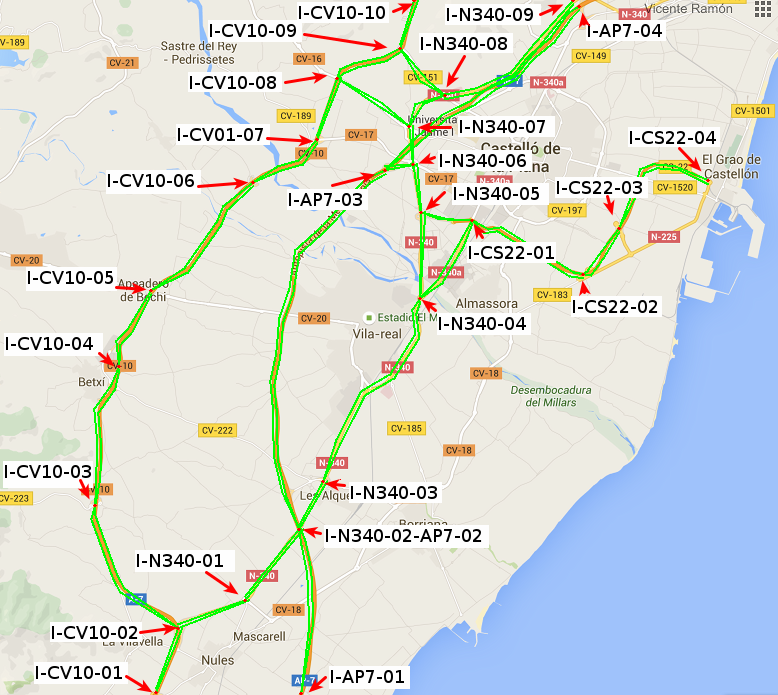
\includegraphics[scale=0.4]{images/map.png} 
  \caption{Road network map}
  \label{map}
\end{figure}

\begin{figure}[!ht]
  \centering
  \includegraphics[scale=0.4]{images/graph.png} 
  \caption{Road network graph}
  \label{graph}
\end{figure}

\section{Results}

The goal of this tests is to show how the smart cars behave in a dynamic environment. To see how the percentage of them affects the system, the data of all the segments have been retrieved. This data contains the number of cars, the service level, the maximum speed for that segment and the current speed.

The current speed is dependent of the service level of the segment and is the maximum allowed speed at that point in time. Figure \ref{traffic} (a bigger version of this figure can be found at Figure \ref{ap:traffic}) shows a plot for 16 hours for one of the most demanding segments. It is easy to see that the more cars there are in the segment, the slower the current speed. In this segment a extreme situation is never reached, but gives a good overview of how to used the output data from the MAS.

With this data, the best results we can take is the average current speed for all segments on a given simulation, and we can compare the 11 simulations to see how the system has performed. This will give us a very good idea of how the system becomes more stable and efficient the more smart cars there are. The results have been plotted in Figure \ref{vcurrent} (a bigger version of this figure can be found at Figure \ref{ap:vcurrent})  and, as expected, the system behaves better when we increase the percentage of smartcars.

The peak at 8:00 is caused because prior to that there are no cars on the simulator, so they can move freely and at maximum speed at first. After that we can see a low speed area when the event manager starts adds all the agents, because all the agents are added in valid intersections and the system has not been stabilized some segments start to lower its service level. After that the system stabilizes with a low number of vehicles per segment, allowing full speed on most of them. And then, when cars are added the system fully stabilizes and smartcars start to dynamically adjust their routes. The average number of cars per segment can be seen in Figure \ref{numCars} (a bigger version of this figure can be found at Figure \ref{ap:numCars}) .

We can see that in both Figures, when the system does not have any smart node, it behaves really poorly. Its average speed as seen in Figure \ref{vcurrent} is way lower than any other case. It is surprising that even with a 10\% of the cars being aware of the traffic, the average speed has an improvement of 3 km/h. This is also obvious in the average number of cars per segment, Figure \ref{numCars}, when we can see that when there is a raise on the proportion of smartcars, there are less cars on the network. That is due to them reaching faster their destinations.

\begin{figure}[!ht]
\hspace{-1.5cm}% Move it slightly to the left
  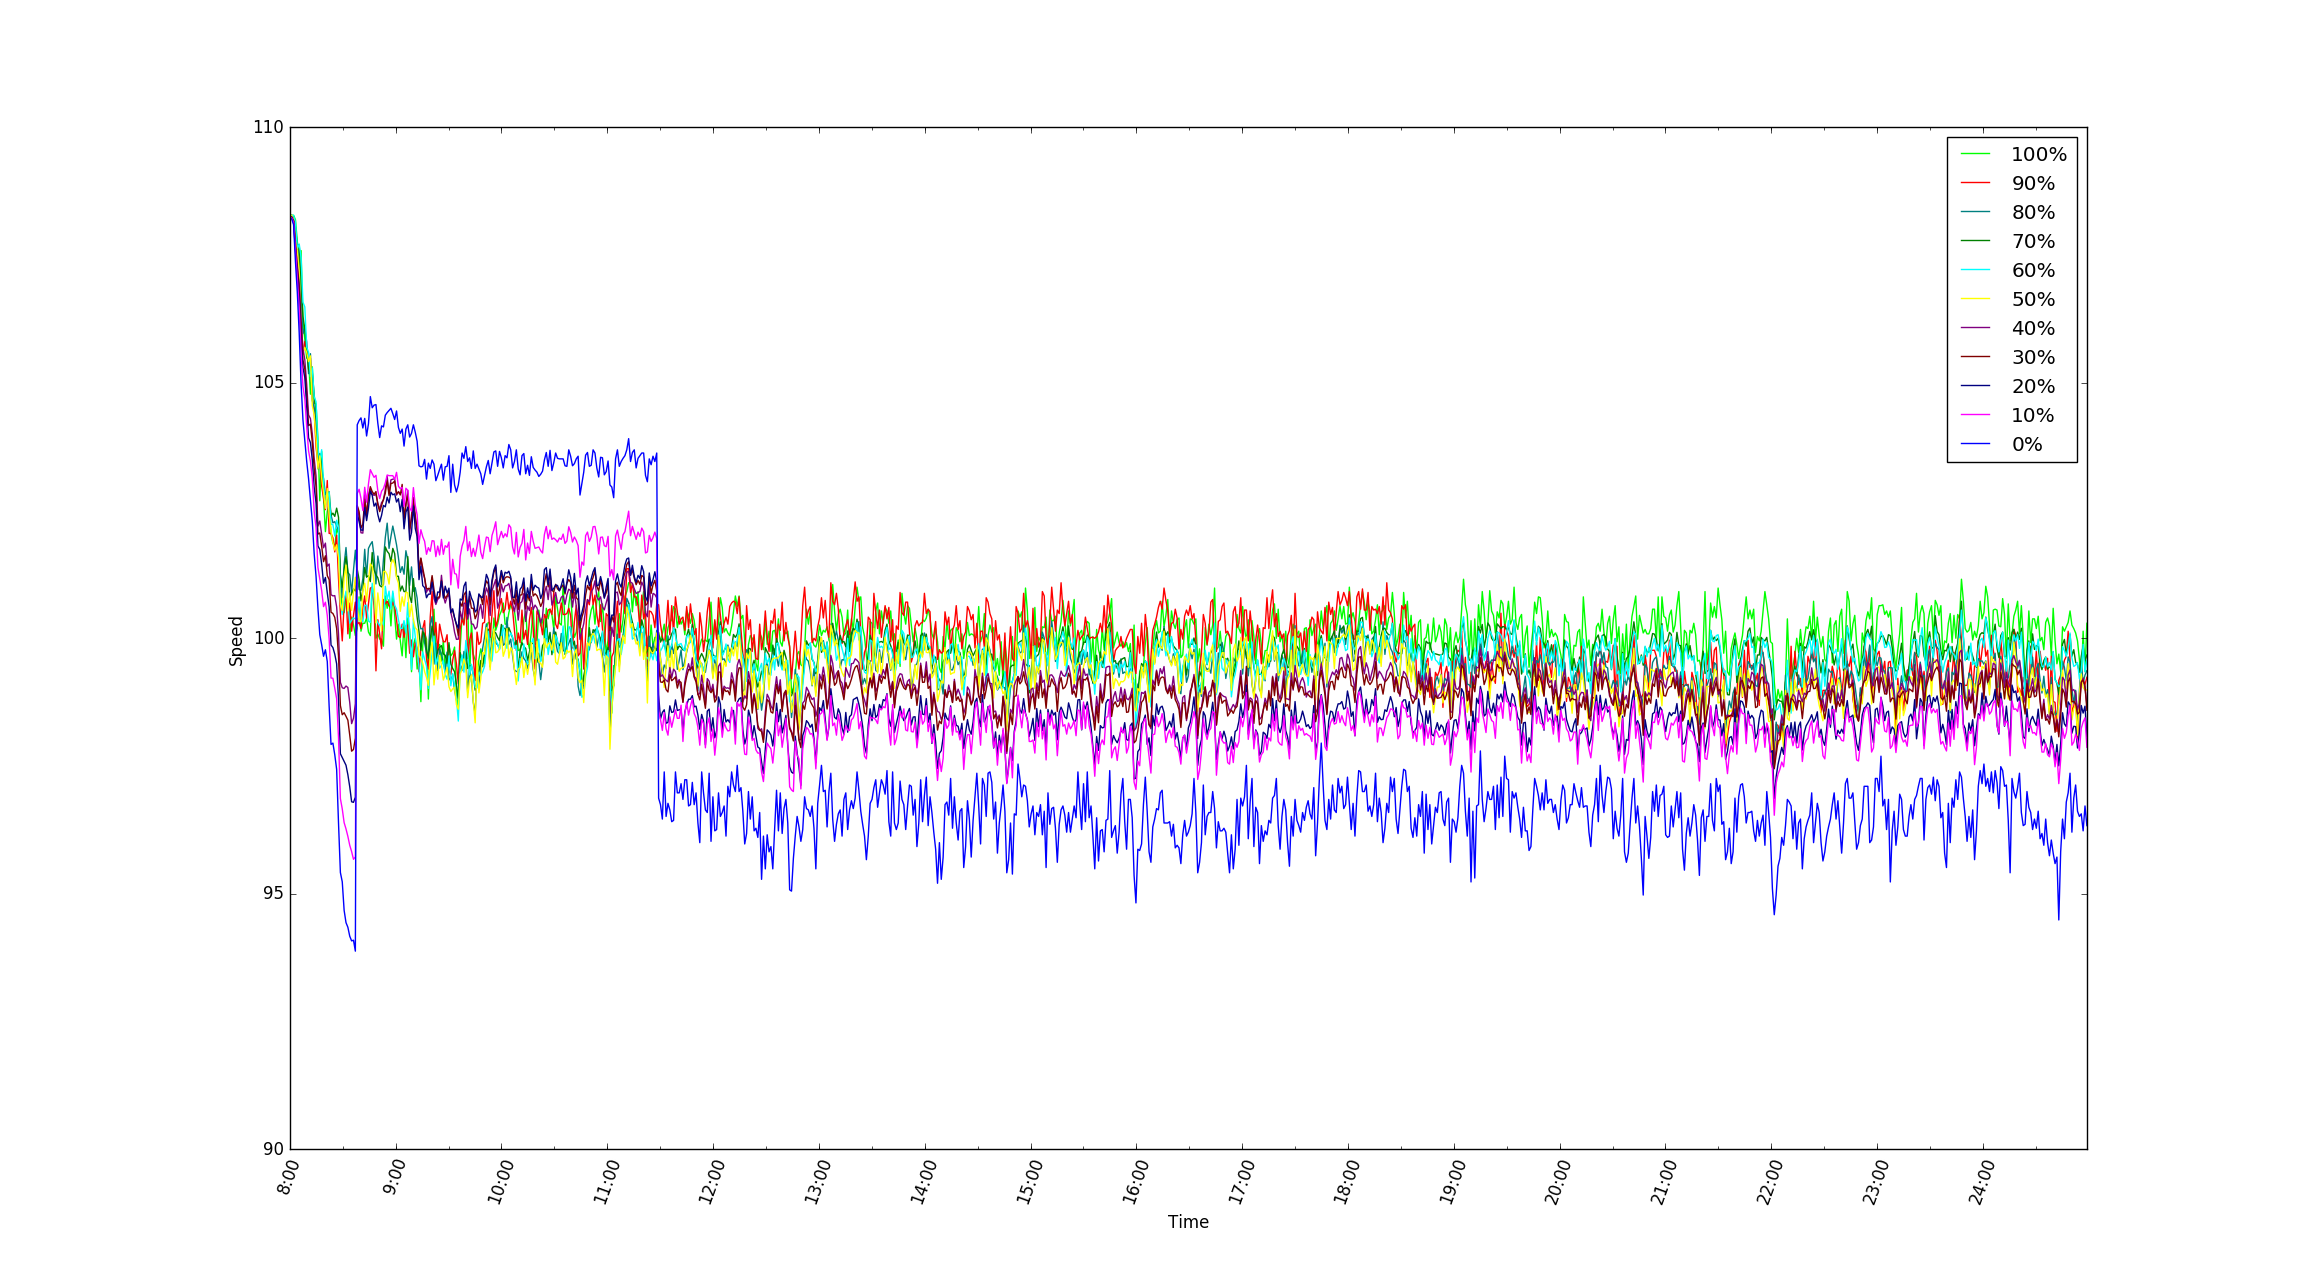
\includegraphics[scale=0.3]{images/Speed.png}
  \caption{Results for the mean current velocity speed}
  \label{vcurrent}
\end{figure}

\begin{figure}[!ht]
\hspace{-1.5cm}% Move it slightly to the left
  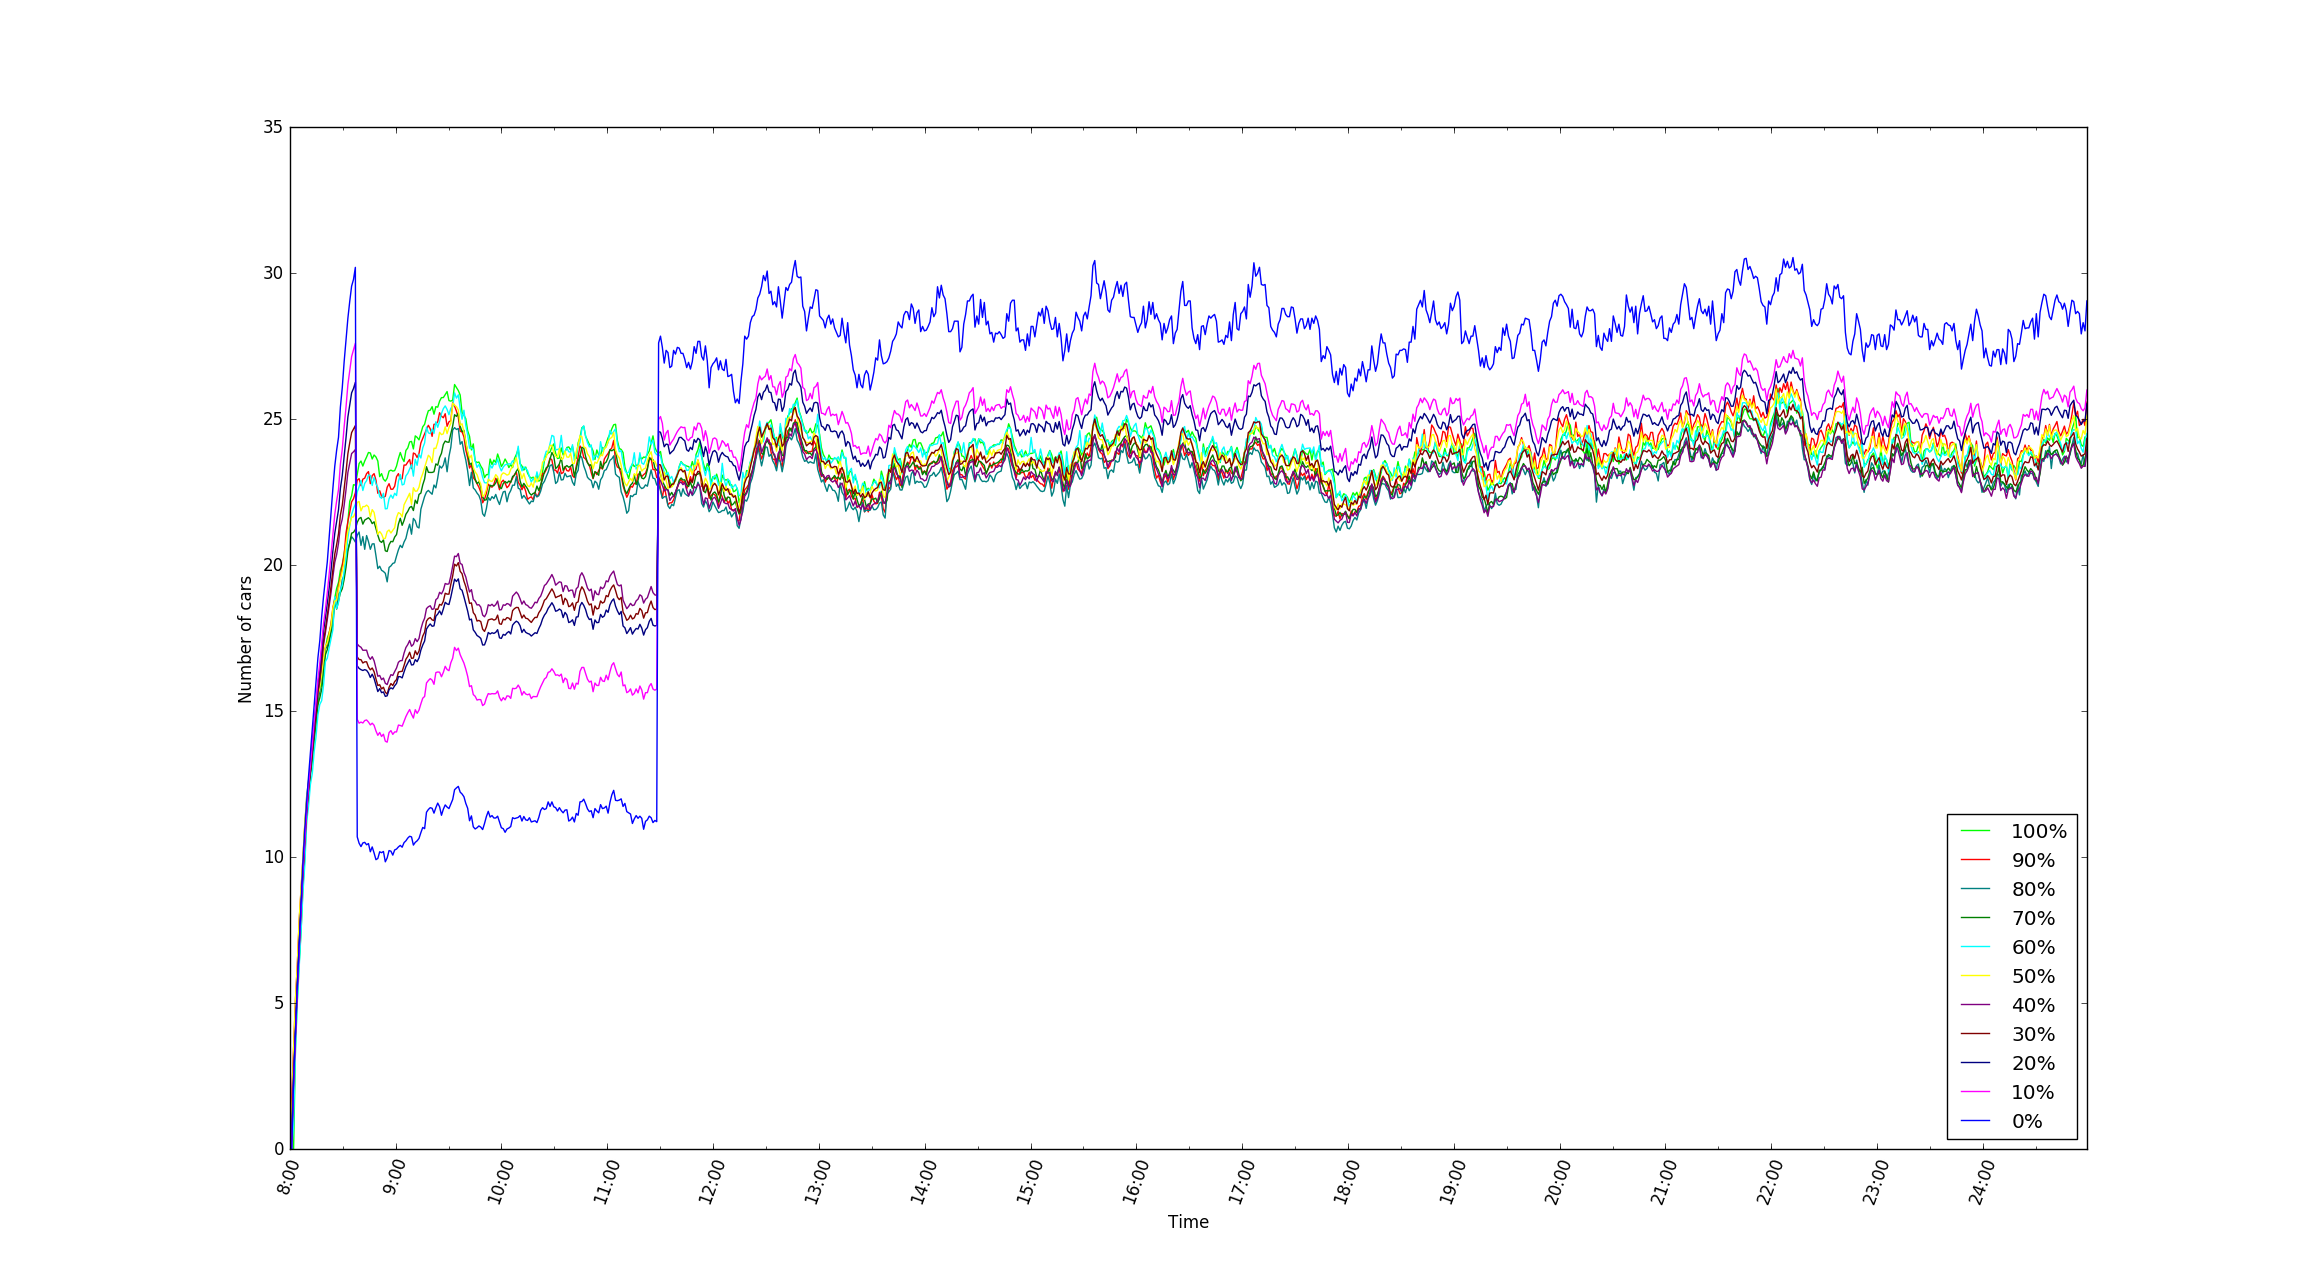
\includegraphics[scale=0.3]{images/Num_cars.png}
  \caption{Results for the mean current number of cars}
  \label{numCars}
\end{figure}

\begin{figure}[!ht]
\
  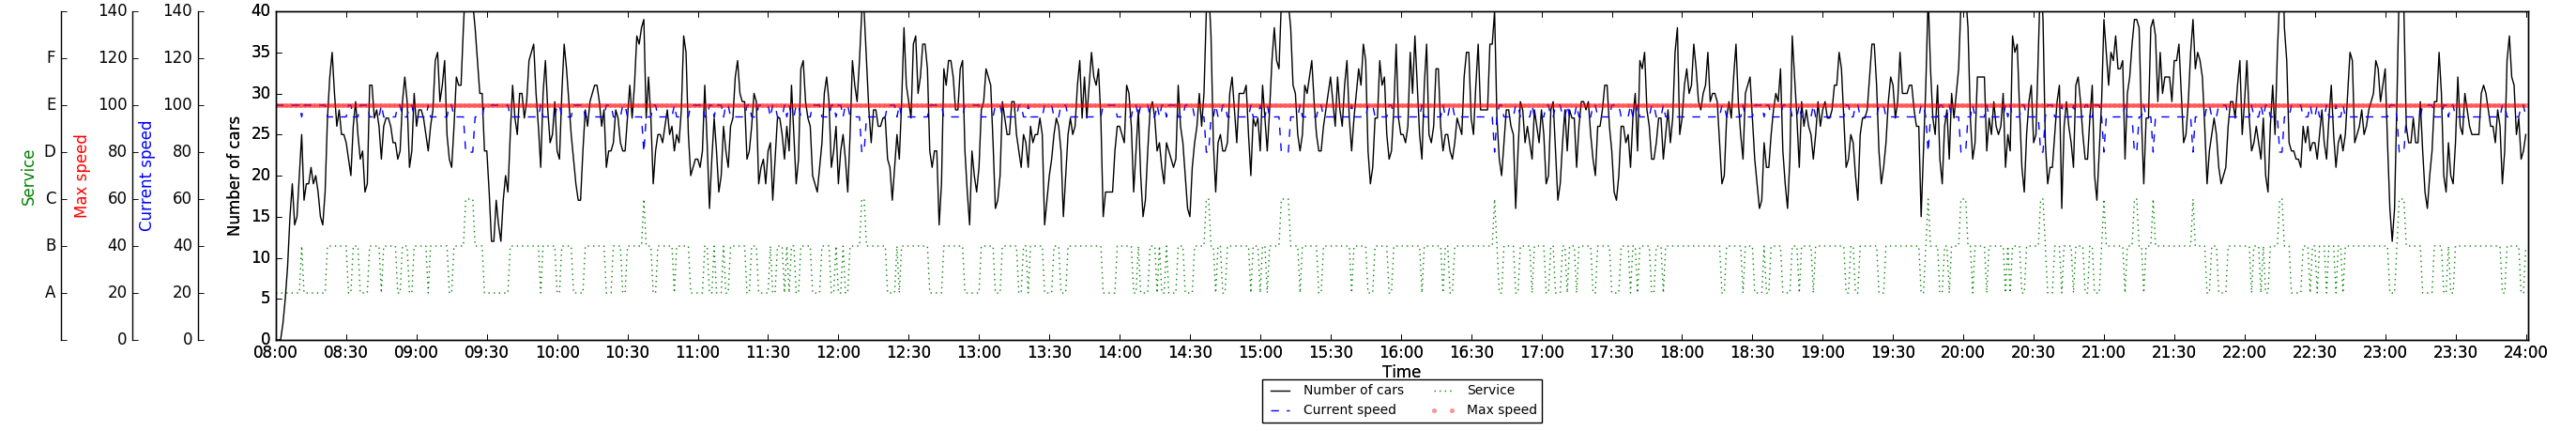
\includegraphics[scale=0.2]{images/cs2201.png}
  \caption{Traffic on the segment CS-22-01}
  \label{traffic}
\end{figure} % Tested the system

\chapter{Conclusions and future work}
\label{ch:conclusions}

\section{Personal experience}

This project was incredibly challenging, developing all the required models for the distributed multiple agent simulator took me longer than anticipated. This was also the most ambitious project I have ever developed, and I had to use every technique that I learned on the bachelor and on the master.

As mentioned in previous chapters, I used the JADE library and open source implementation of a distributed communication framework. While working with it I found two bugs that I had reported, and many times the only workaround until the fix came was simply changing the source code, recompiling and carrying on. The documentation on this library is very good, but for advanced MAS it was a little bit short.

I spent a big quantity of this projects time optimizing the system to support as many cars as possible, finding the limitations of this library at every corner. The biggest limitation that I found was how to deliver that many messages in a timely manner from the TimeKeeper agent to the rest of the agents to synchronize the simulation time, and that was my bottleneck for many weeks.

Also, since the GUI is updating itself very fast, I had to use all the tricks in the manual to make it as efficient as possible, and I had to learn how the most advanced swing techniques had to be applied.

Another big problem I had were the communication ontologies, I had to create unique ontologies so that the communication between agents could easily be extended.

The development of the routing algorithms was also challenging, but I did learn a lot about graphs and its representation, I even made my own system to store that graph in a human readable way to a file. The smart algorithm was very difficult at first, I tried and failed with many implementations of that algorithm that finally weren't good and simple enough.

In conclusion, I am incredibly proud of this project, it is modular, distributed, open source and I have employed many new technologies that I had never used before.

\section{Conclusions}

As has been shown in Chapter \ref{ch:tests} even with a very little userbase, big gains can be achieved. This kind of technology not only helps those that use it, although they are the more benefited, but helps every user of the network. The traffic becomes more fluid, travel times shorten and, because cars spend less time on the road, the level of pollution decreases.

\section{Future work}

Ideally, in the future a real life scenario can be set to test the results of this thesis, with just a little bit of hardware this could be tested on a small section of the network.

Another model that could be tested on this MAS, now that is finished, is an algorithm that predicts which segments the cars that are in the network are going to take, and how that will affect the service level in the future. If the system were to know all the paths that all the cars want to take, further improvements could be achieved since no predictions would have to be made. But this last idea creates a privacy conflict and is why it has not been studied further.



 % Hopefully the last chapter

%\input{Chapters/Chapter2} % Background Theory 

%\input{Chapters/Chapter3} % Experimental Setup

%\input{Chapters/Chapter4} % Experiment 1

%\input{Chapters/Chapter5} % Experiment 2

%\input{Chapters/Chapter6} % Results and Discussion

%\input{Chapters/Chapter7} % Conclusion

%% ----------------------------------------------------------------
% Now begin the Appendices, including them as separate files

\addtocontents{toc}{\vspace{2em}} % Add a gap in the Contents, for aesthetics

\appendix % Cue to tell LaTeX that the following 'chapters' are Appendices

\chapter{Bigger figures}

\begin{figure}[!ht]
  \centering
  \begin{adjustbox}{angle=90} 
  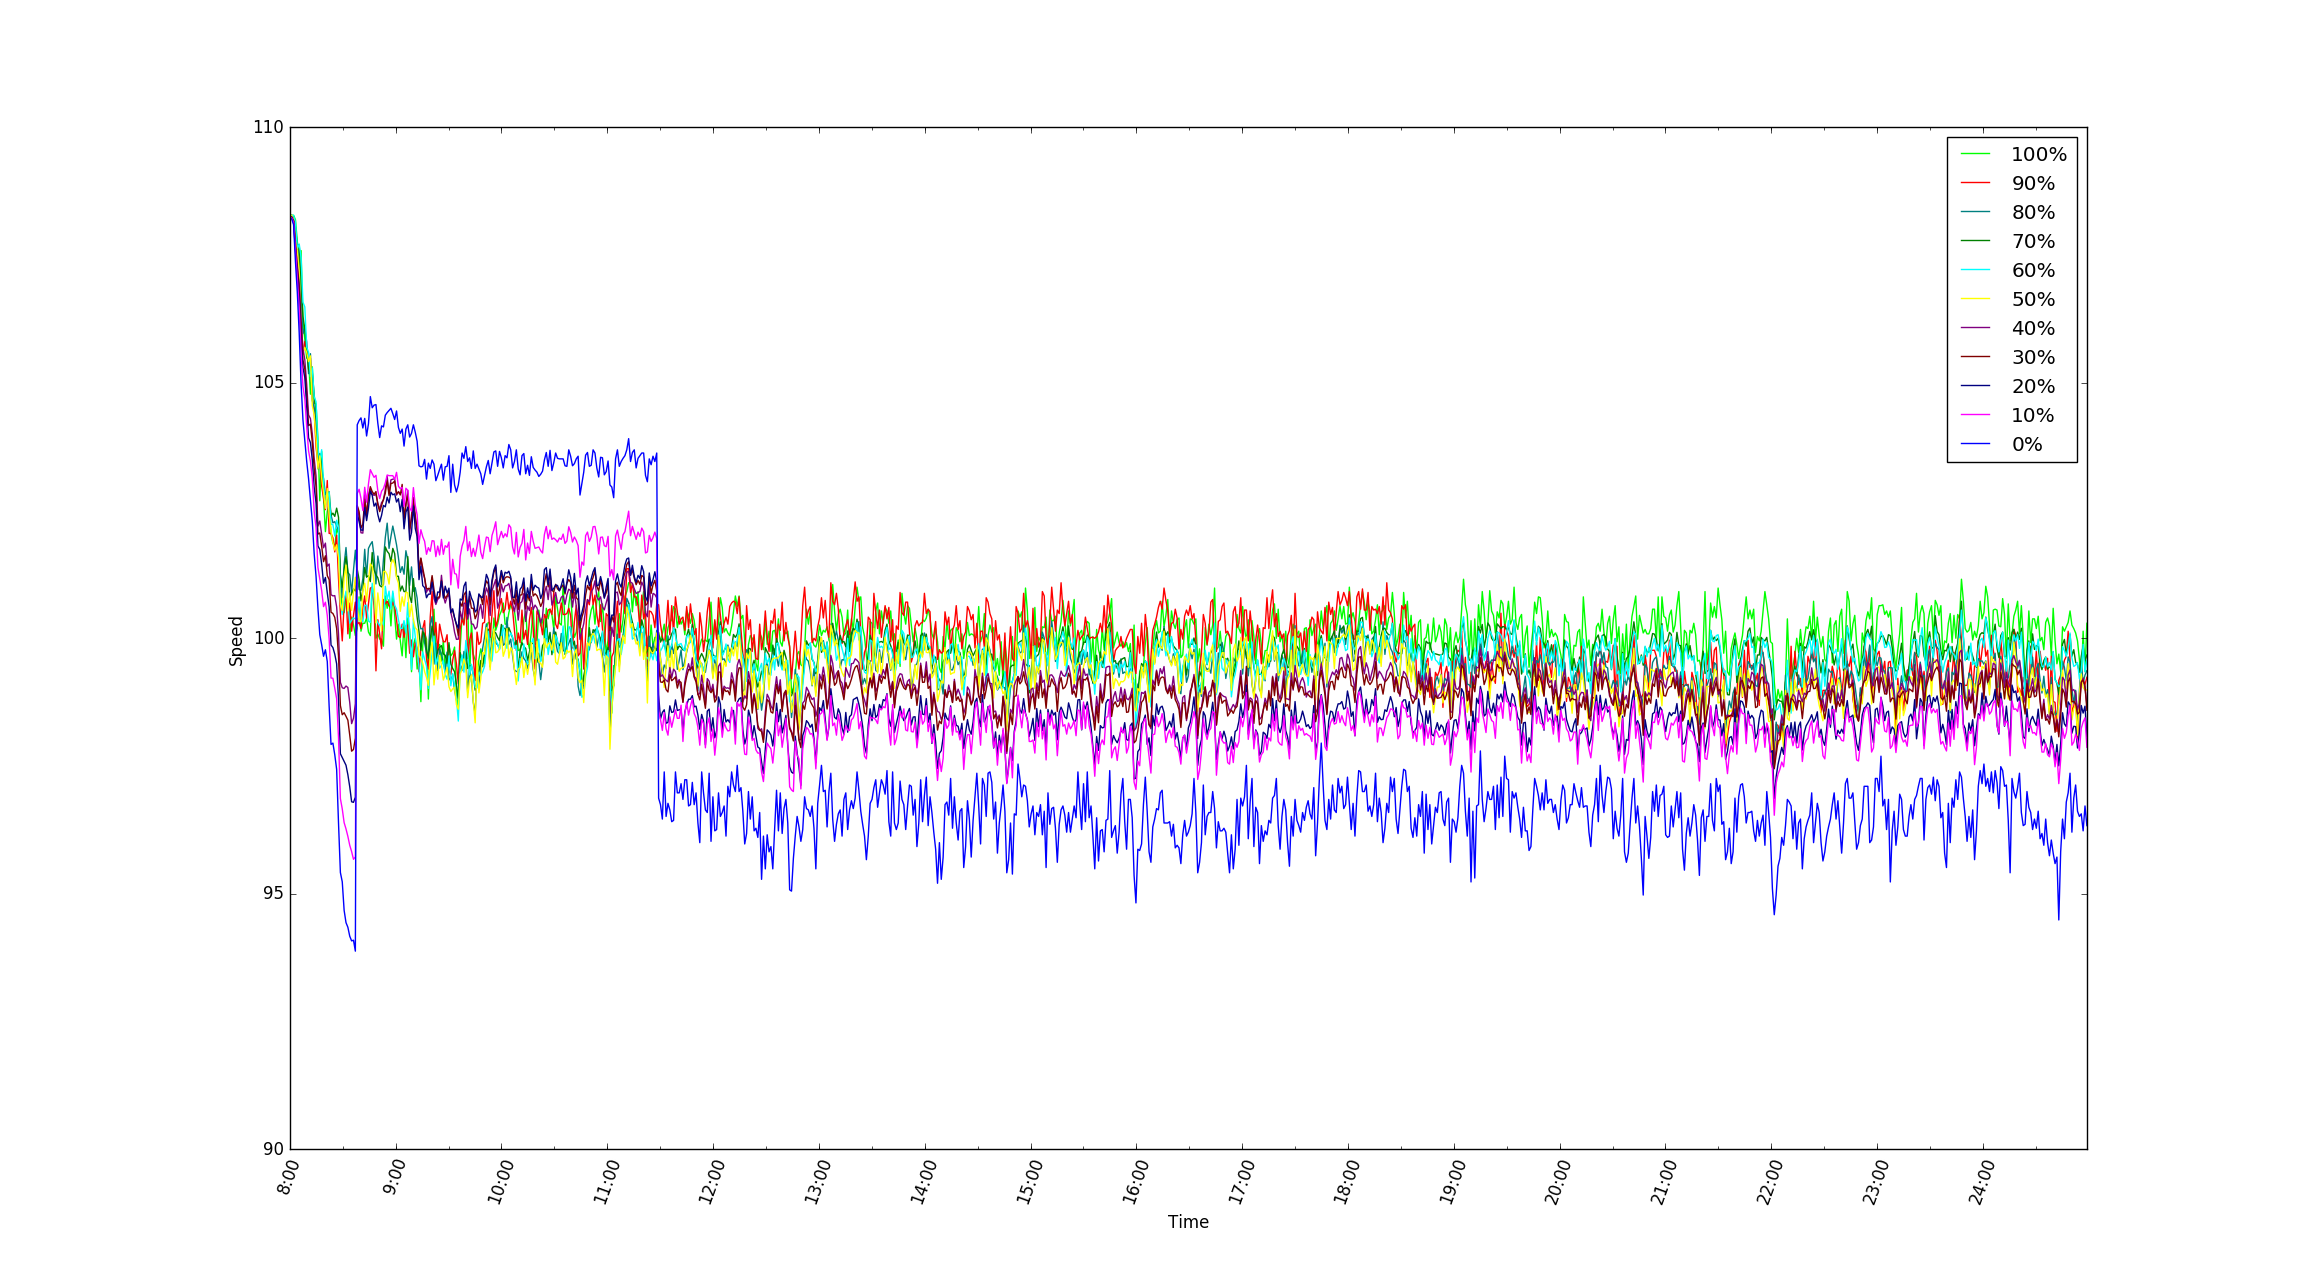
\includegraphics[scale=0.4]{images/Speed.png}
  \end{adjustbox}
  \caption{Results for the mean current velocity speed}
  \label{ap:vcurrent}
\end{figure}

\begin{figure}[!ht]
  \centering
  \begin{adjustbox}{angle=90} 
  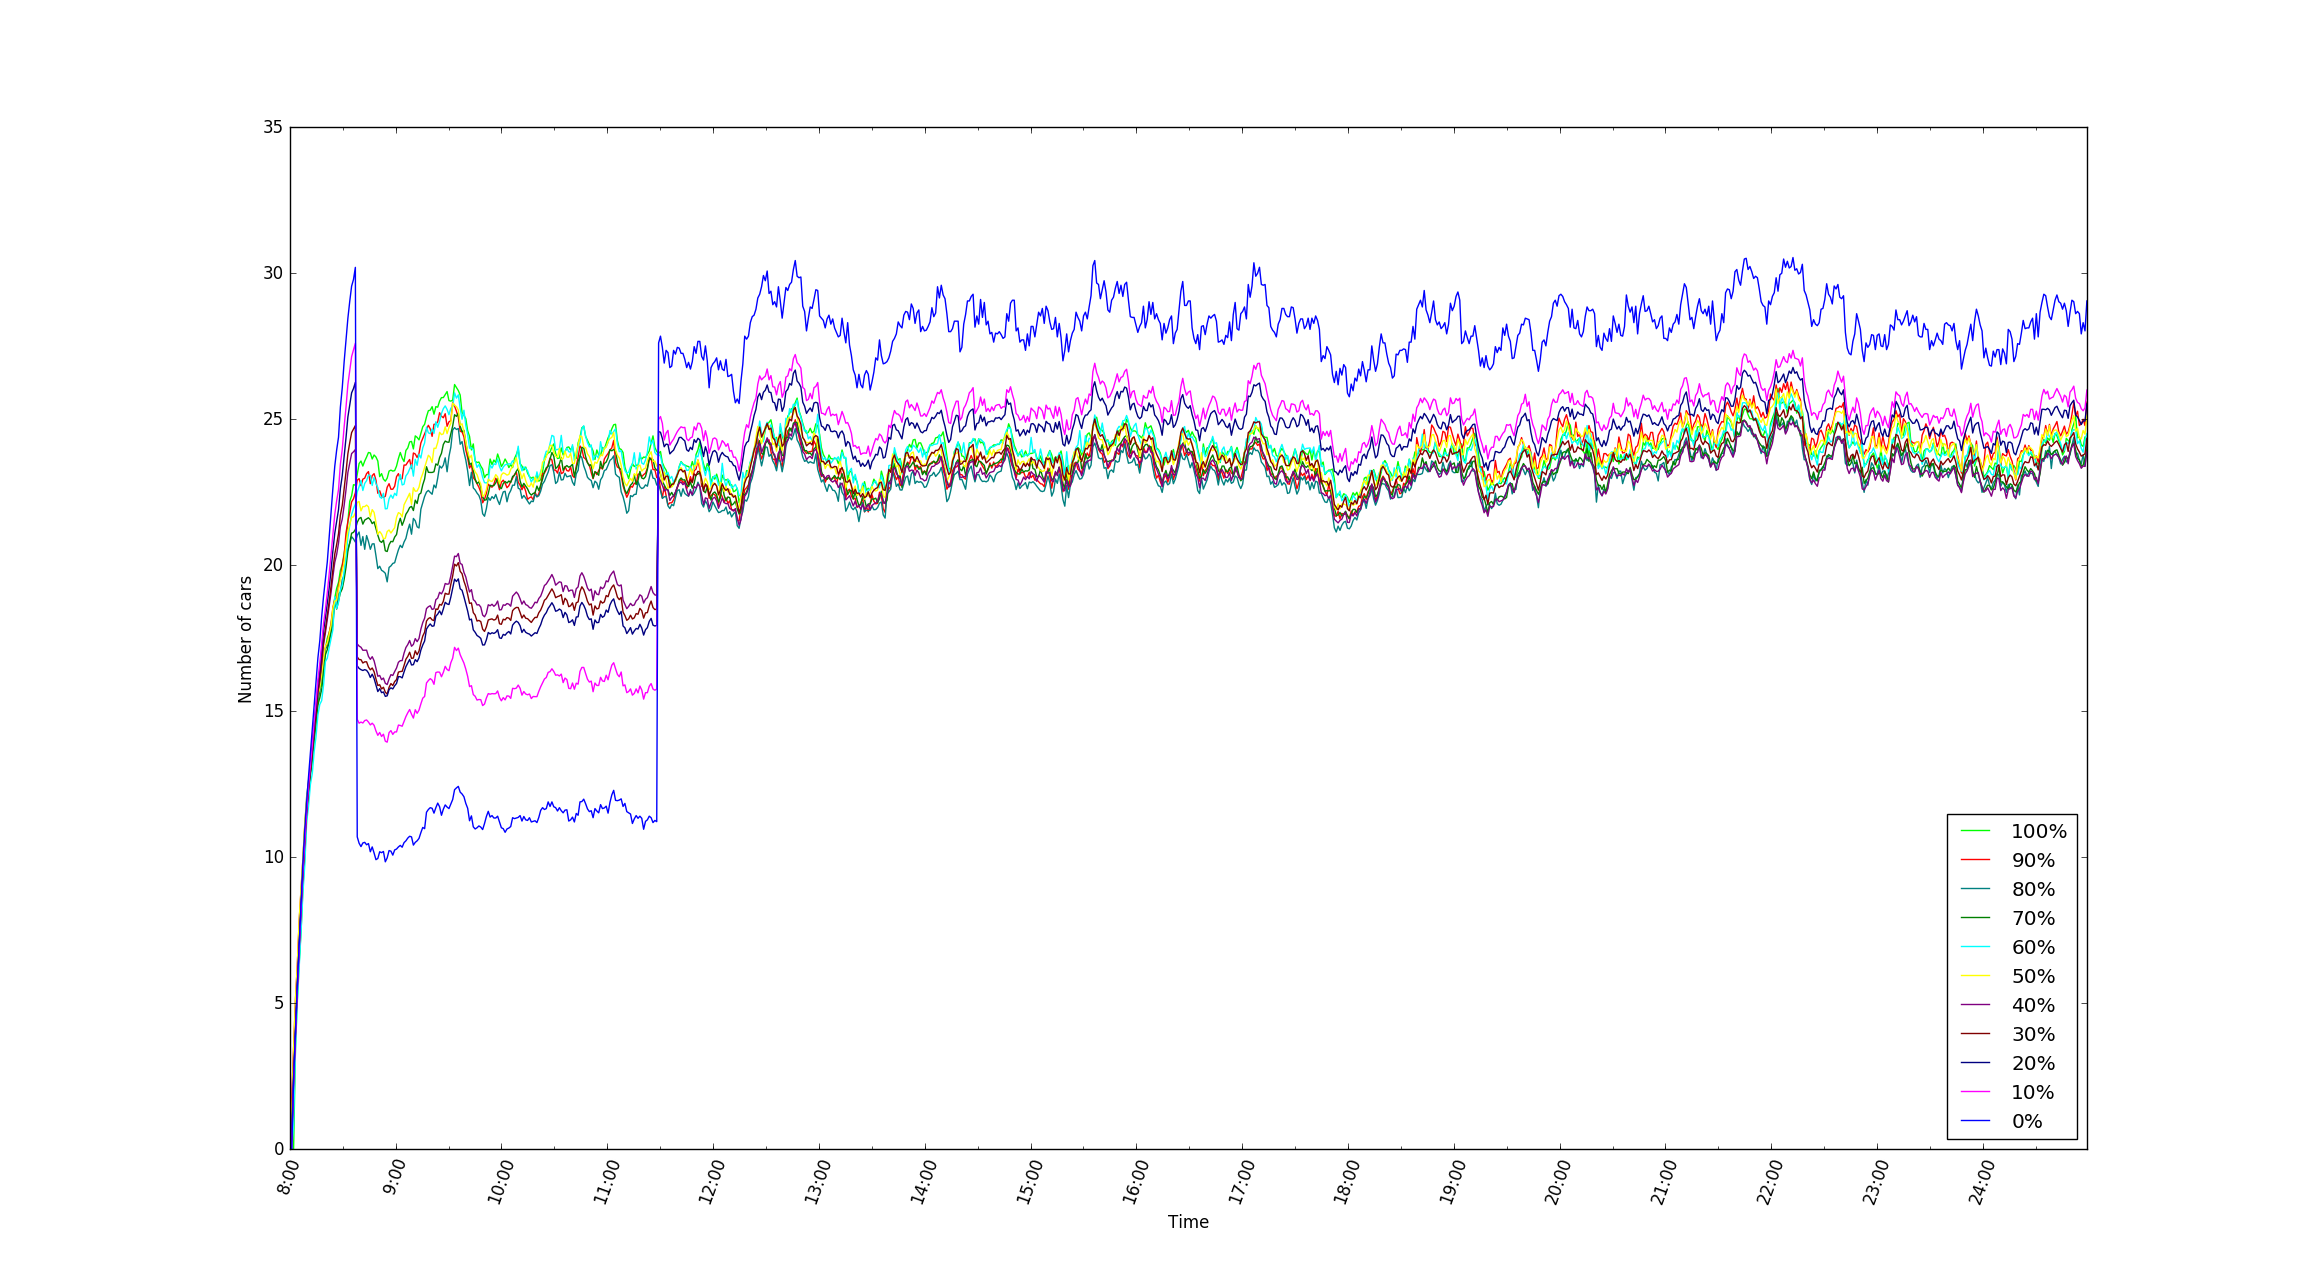
\includegraphics[scale=0.4]{images/Num_cars.png}
  \end{adjustbox}
  \caption{Results for the mean current number of cars}
  \label{ap:numCars}
\end{figure}

\begin{figure}[!ht]
  \centering
  \begin{adjustbox}{angle=90} 
  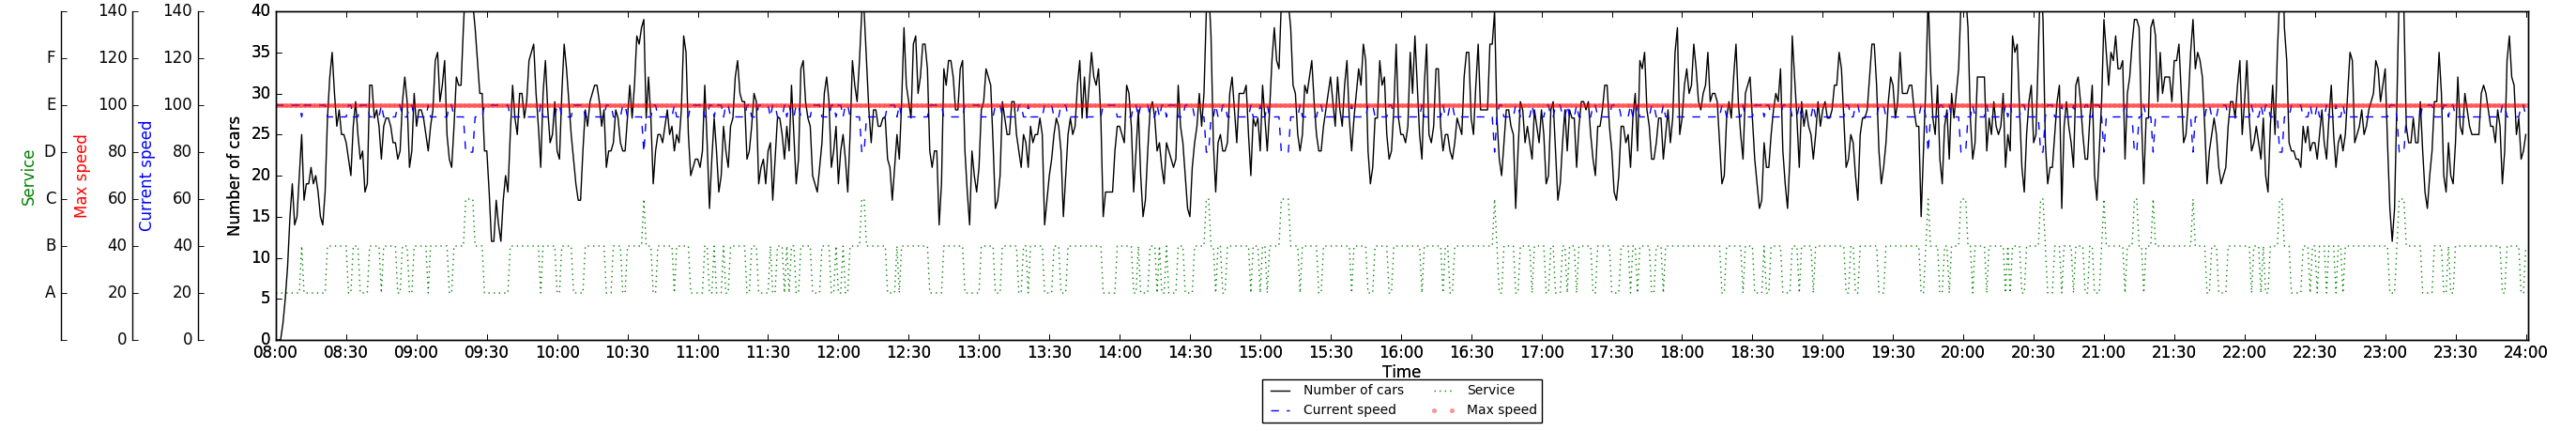
\includegraphics[scale=0.3]{images/cs2201.png}
  \end{adjustbox}
  \caption{Traffic on the segment CS-22-01}
  \label{ap:traffic}
\end{figure}	% Appendix Title

%\input{Appendices/AppendixB} % Appendix Title

%\input{Appendices/AppendixC} % Appendix Title

\addtocontents{toc}{\vspace{2em}}  % Add a gap in the Contents, for aesthetics
\backmatter

%% ----------------------------------------------------------------
\label{Bibliography}
\lhead{\emph{Bibliography}}  % Change the left side page header to "Bibliography"
\bibliographystyle{unsrtnat}  % Use the "unsrtnat" BibTeX style for formatting the Bibliography
\bibliography{Bibliography}  % The references (bibliography) information are stored in the file named "Bibliography.bib"

\end{document}  % The End
%% ----------------------------------------------------------------